
\chapter{Architecture du projet}

   
\section{Code fourni par le client}

Le code fourni par le client se compose de deux packages. Il 
nous a été spécifiquement demandé de travailler avec OpenCV3. 
Pour nous aider à utiliser OpenCV, nous avons utilisé 
\cite{ref3}.

\subsection{hl\_communication}

Le premier package \textbf{hl\_communication} contient les 
classes nécessaires à la lecture des messages des robots.
\bigskip

Nous avons dans ce package les multiples fichiers 
\textit{.proto} décrivant l'architecture des messages. 

L'architecture globale des messages est disponible en 
annexe~\ref{annexe}, page~\pageref{annexe}. La 
Figure~\ref{fig:message} ci-dessous nous montre une version 
simplifiée avec seulement les éléments des messages que nous 
utilisons.
\bigskip

Un message se compose de deux parties essentielles : les 
messages du \textbf{Game\_Controller} et ceux des robots. La 
hiérarchie de départ du message est contenue dans le fichier 
\textit{wrapper.proto}.
\bigskip

Le \textbf{Game\_Controller GC\_Msg} contient toutes les 
données réelles du match, c'est à dire toutes les données 
envoyées par la table d'arbitrage: le temps, les équipes 
(\textbf{GCTeamMsg}) et leurs robots (\textbf{GCRobotMsg}). 
\bigskip



\begin{figure}[H] 
\centering 
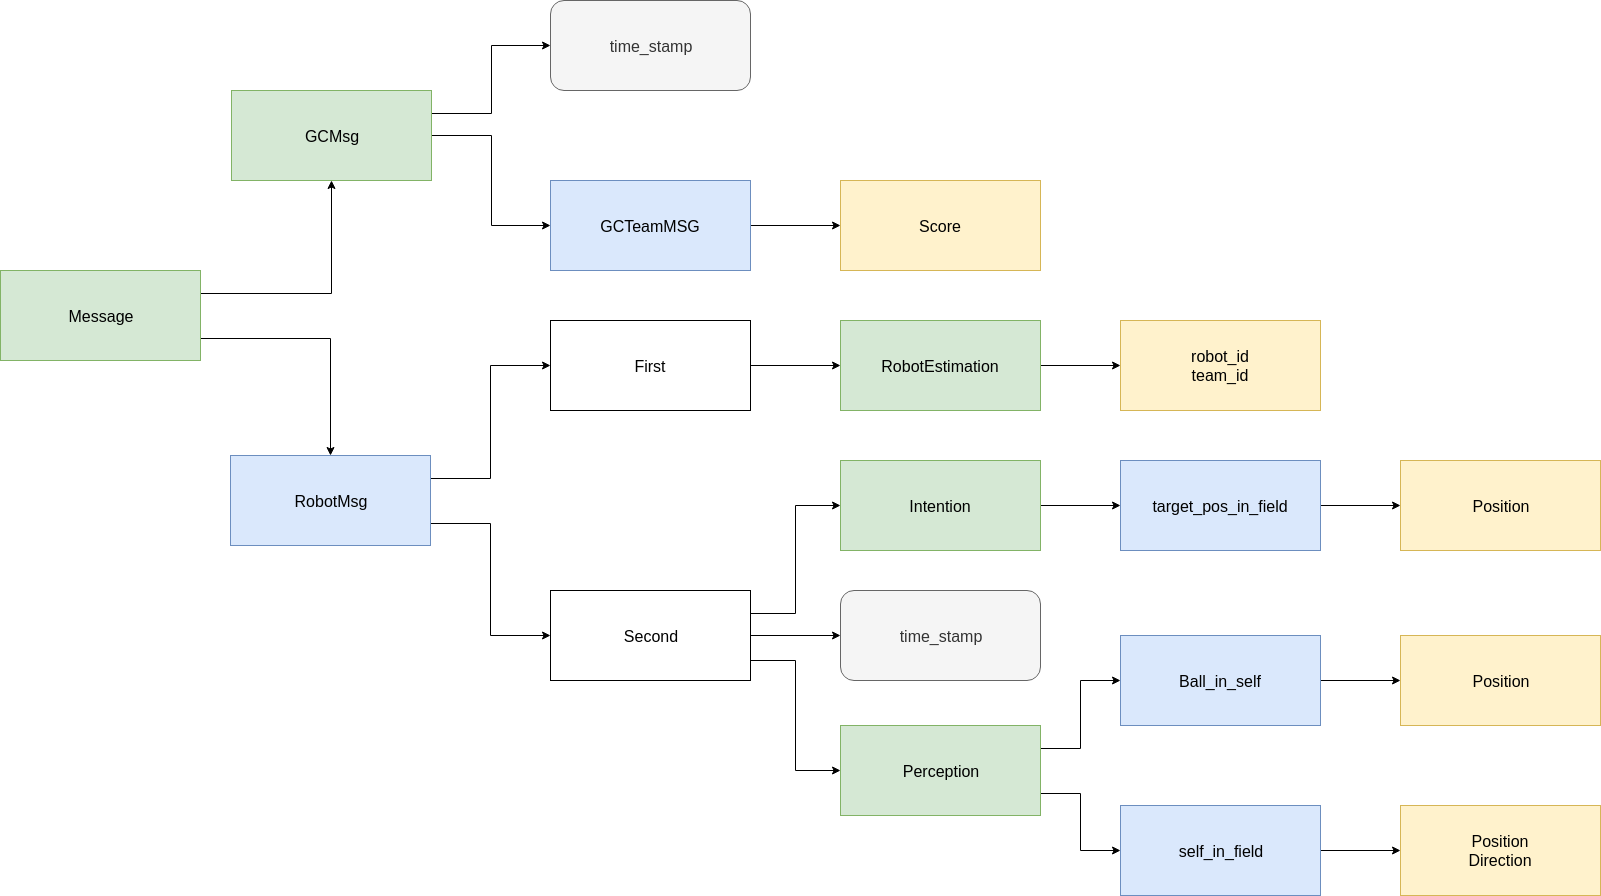
\includegraphics[scale = 0.24]{images/shortmessage.png}
    \caption{Architecture des messages}
    \label{fig:message}
    {\textit{En vert, les noms se rapportant aux fichiers
    proto. En bleu, ce sont les sous-ensembles des messages et
    en jaune les éléments du match que nous récupérons. }}
\end{figure} 


Dans ces messages nous récupérons le numéro des équipes et le 
score.
Nous recevons également un message \textbf{Robot\_Msg} par
robot. Dans notre programme nous traitons plusieurs éléments
de ces messages :
\begin{itemize}
    \item le \textbf{time\_stamp} pour mesurer le temps écoulé
    depuis l'envoi du message;
    \item le \textbf{Robot\_Estimation} : qui nous donne son 
    numéro d'équipe et de robot;
    \item la \textbf{Perception} du robot : on récupère ici la
    position et la direction du robot
    (\textit{self\_in\_field}) et de la balle 
    (\textit{ball\_in\_self});
    \item Enfin, l'\textbf{Intention} du robot est utilisé 
    pour avoir sa position souhaitée 
    (\textit{target\_pose\_in\_field}).
    
\end{itemize}
\bigskip

Les principales fonctions que l'on utilise de ce package sont 
contenues dans la classe \textbf{MessageMonitoring} dont nous 
utilisons principalement la fonction 
\textbf{getStatus(time\_stamp)} qui nous donne le message 
correspondant à un certains temps \textit{time\_stamp}.
\bigskip

\subsection{hl\_monitoring}

Ce second package contient essentiellement le 
\textbf{MonitoringManager} qui nous permet de rythmer 
l'avancée de la vidéo. 
\bigskip

Tout d'abord, il lit le fichier de configuration 
\textit{match\_settings.json} puis 
\textit{replay.json/live.json} qui contient le nom du binaire 
où l'on récupère les messages des robots, les informations sur
les caméras et leur vidéos et enfin un booléen pour savoir si 
on est en replay ou en live.

C'est également lui qui va initialiser le 
\textbf{MessageManager} vu précédemment. Tant que ce manager 
fonctionne, il va récupérer l'image à un temps donné de la 
vidéo. 
\bigskip

La classe \textbf{Field} permet d'afficher les lignes du 
terrain grâce à la fonction \textbf{tagLines}.
\bigskip

\begin{figure}[H] 
\centering 
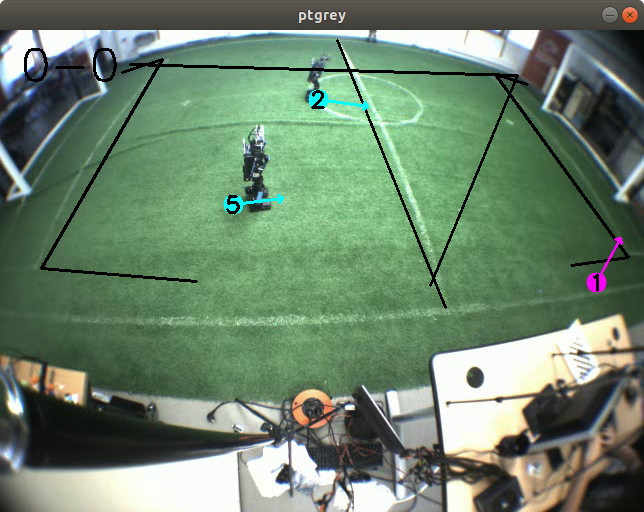
\includegraphics[scale = 0.3]{images/test2.png}
    \caption{Test sur l'affichage des lignes du terrain}
    \label{fig:field}
\end{figure} 

 Elle nous permet de vérifier le bon fonctionnement de la 
 calibration de la caméra. Par exemple, dans le cas de la 
 vidéo \textit{ptgrey.avi} tournée le 20/02/2019, les lignes 
 du terrains ne correspondent pas à la réalité. 
 
 Nous pouvons voir sur la photo que la ligne de la zone du 
 gardien proche du joueur 1 en rose est mal placée. En 
 revanche, même si la ligne est mal placée, la position du 
 robot est bien placée par rapport à la ligne.
\bigskip

\newpage

\textbf{Hl\_monitoring} contient toutes les fonctions de 
calibration de la caméra, dont l'outil 
\textit{static\_calibration} (qui nous permet de calibrer une 
caméra une fois que l'on a récupéré ses paramètres 
intrinsèques). Il contient aussi la fonction 
\textbf{fieldToImg}, qui transforme des positions du plan réel
au plan de l'image en fonction des paramètres de la caméra. 
\bigskip

Le package \textbf{hl\_monitoring} contient aussi
\textit{basic\_monitoring}. C'est un exécutable permettant de 
tester tout ce qui nous a été fourni par le client. C'est dans
ce fichier que nous avions fait nos premiers tests d'affichage
avant d'en créer un nous-même.

\section{Architecture du code}

Nous avons ajoutés deux packages à ceux fournis par le client.

D'une part nous avons \textbf{annotateImage} qui nous permet 
d'annoter la vidéo et de l'afficher d'une façon très basique 
et d'autre part \textbf{Interface} qui nous permet d'afficher 
la vidéo avec une interface utilisateur et de changer les 
annotations en cours de lecture.
\bigskip

L'annotation d'image se compose de différentes classes:
\begin{itemize}
    \item des classes outils telles que \textbf{Position} ou 
    \textbf{Direction} : nous permettant de mieux gérer les 
    éléments récupérés dans les logs;
    \item les classes \textbf{RobotInformation} et 
    \textbf{Team} : Team se compose d'une map de
    RobotInformation, elle est essentielle pour différencier 
    les robots lors de la réception des messages; 
    RobotInformation nous permet donc de stocker le dernier 
    message de chaque robot et d'autres informations utiles 
    aux annotations (la trace principalement);
    \item la classe \textbf{Annotation} qui contient une 
    fonction par annotation qu'il est possible d'ajouter.
\end{itemize}
\bigskip

Le fichier principal de annotateImage est 
\textit{main\_annotateImage}, il permet de lancer la vidéo et 
d'annoter la vidéo grâce aux deux fichiers de configuration 
\textit{match\_settings.json} et 
\textit{annotation\_settings.json}. Le détail des choix 
possibles pour ces fichiers se fera dans la partie suivant, 
fonctionnalités implémentées.
\bigskip

Enfin, nous pouvons retrouver trois fichiers de tests que l'on
détaillera dans la partie appropriée.
\bigskip

\newpage

L'interface a été conçue à partir de l'API Qt. Elle est 
composée de différentes classes qui héritent de classes Qt :
\begin{itemize}
    \item \textbf{MainWindow} : hérite de QMainWindow,
    représente la fenêtre principale de l'interface;
    \item \textbf{TeamPanel} et \textbf{RobotPanel} : héritent
    de QWidget, ces deux classes nous permettent de faire
    savoir l'état d'une annotation pour chaque robot via des
    QLabel;
    \item \textbf{ChoiceDialog} : hérite de QDialog,
    représente la fenêtre pop-up servant à modifier les choix
    d'Annotation;
    \item \textbf{ChoiceComboBox} : hérite de QWidget, permet
    de sélectionner le numéro d'une équipe et d'un robot.
    Créée par choix de factorisation puisque ce mode de choix
    était présent 3 fois dans ChoiceDialog.
\end{itemize}
\bigskip

Le fichier principal \textit{main} permet d'exécuter
l'interface.
\bigskip

Voici donc comment se trouve notre architecture, les deux
packages en haut sont ceux du client et en bas ceux que nous
avons ajoutés :

\begin{figure}[H] 
\centering 
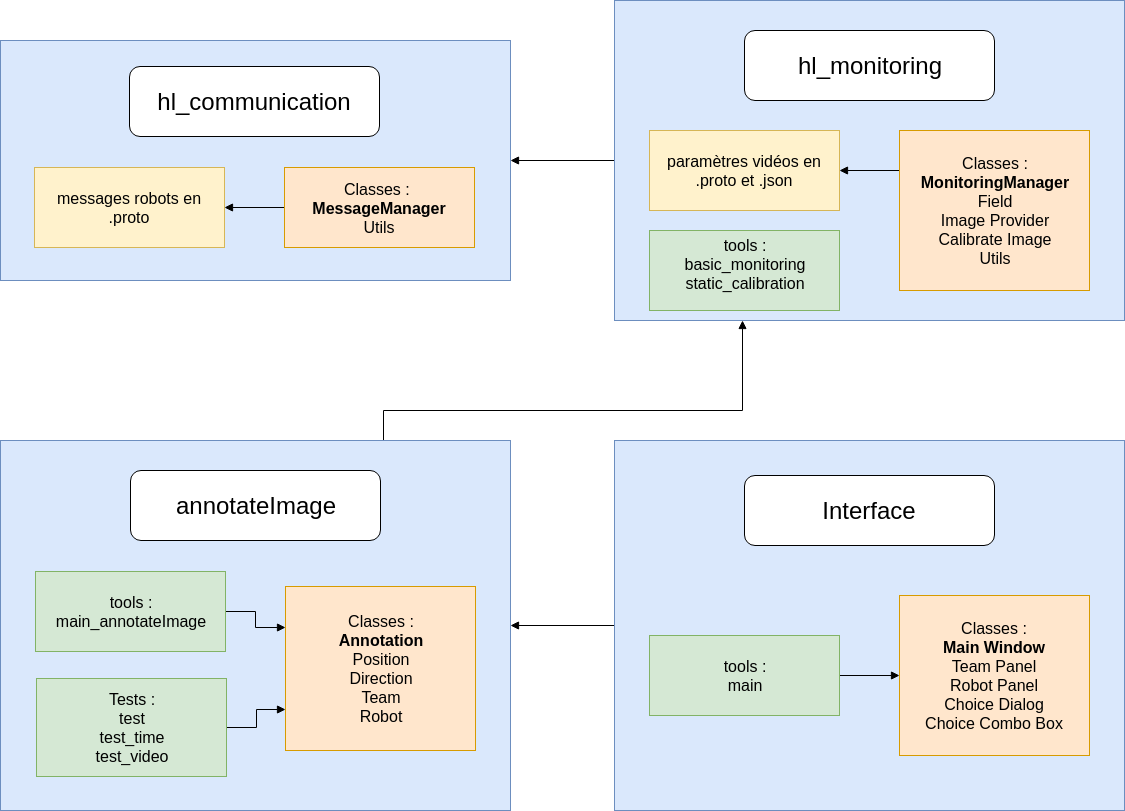
\includegraphics[scale = 0.3]{images/architecture.png}
    \caption{Architecture des packages}
\end{figure} 


\section{Fonctionnement du projet}

Pour expliquer le fonctionnement de notre projet, nous allons 
nous appuyer sur le package \textbf{annotateImage} 
essentiellement, sachant que l'interface fonctionne de la même 
façon avec les outils d'affichage en plus.

\subsection{L'initialisation}

Au lancement de l'exécutable de annotateImage, 
main\_annotateImage, plusieurs fichiers sont indispensables comme
nous pouvons le voir dans la Figure~\ref{fig:entree} ci\_dessous.


\begin{figure}[H] 
\centering 
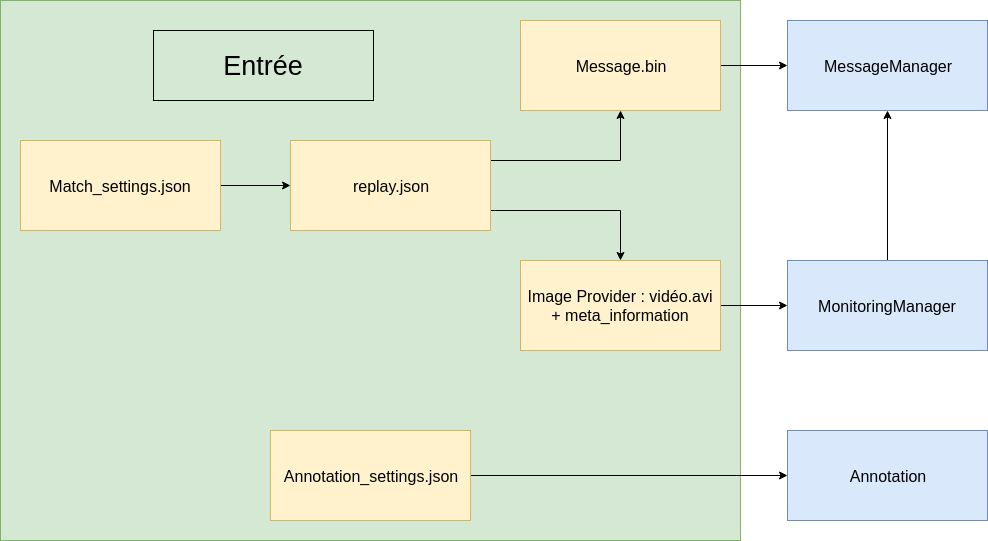
\includegraphics[scale = 0.3]{images/init.png}
    \caption{Entrée et initialisation du programme}
    \label{fig:entree}
\end{figure} 
\bigskip


Le premier, \textit{match\_settings} contient la configuration du
projet qui va être dans un fichier \textit{replay.json} ou
\textit{live.json}.
Le fichier \textit{replay.json} contient d'une part le nom du 
binaire contenant les messages permettant de créer un 
\textbf{MessageManager} et d'autre part le nom de la vidéo à 
traiter, ainsi que celui du binaire contenant les informations de
la caméra associée permettant d'avoir le
\textbf{MonitoringManager}.
\bigskip

Le second fichier indispensable est
\textit{annotation\_settings.json} qui nous permet de créer un 
objet \textbf{Annotation} qui lit le fichier et prend en compte 
tous les paramètres nécessaires à chaque annotation.

À l'initialisation, nous créons également la variable "now" qui 
est un \textit{time\_stamp} et qui rythme l'avancée de la vidéo. 
Il correspond au \textit{time\_stamp} de l'image en cours de 
traitement. 

\subsection{La récupération d'un message}

Avant de nous occuper des images des vidéos, nous récupérons le 
message associé au \textit{time\_stamp}. 

Comme nous pouvons le voir dans la Figure~\ref{fig:log}, nous 
récupérons d'une part les informations de chaque \textbf{Team} 
(le score) et des \textbf{RobotInformation} (le Robot\_Msg). Nous
accédons aux robots à travers leur \textbf{Team}.
\begin{figure}[H] 
\centering 
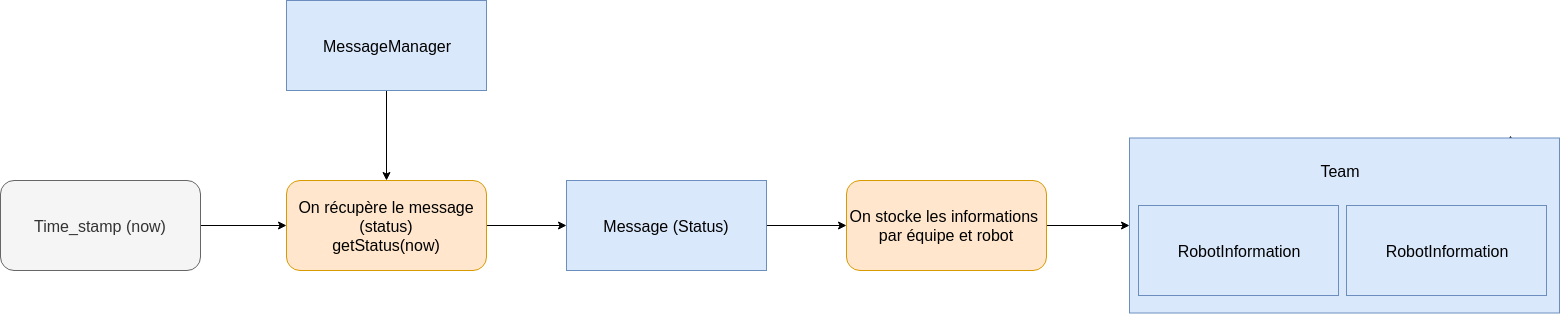
\includegraphics[scale = 0.24]{images/getmessage.png}
    \caption{Récupération des messages}
    \label{fig:log}
\end{figure} 


\subsection{La récupération d'une image}

À chaque \textit{time\_stamp}, nous allons donc récupérer l'image
associé mais il est possible de lancer plusieurs vidéos en
simultané. La récupération d'une image se fait donc comme 
détaillée Figure~\ref{fig:img} : 

\begin{figure}[H] 
\centering 
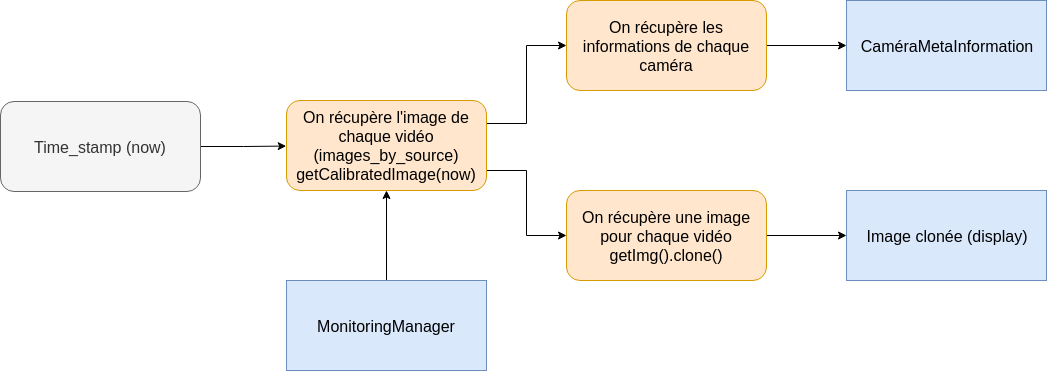
\includegraphics[scale = 0.3]{images/getimage.png}
    \caption{Récupération des images}
    \label{fig:img}
\end{figure} 

Nous récupérons d'abord une std$::$map avec une image par
vidéo puis nous récupérons une image et les meta-informations
de la caméra associé. L'affichage se fait donc image par image
pour chaque vidéo, c'est ce qui permet d'afficher deux vidéos
en simultané.

\newpage

\subsection{L'annotation sur l'image}

Une fois que tous tous les éléments ont été recueillis, nous
pouvons annoter l'image comme on le voit dans la 
Figure~\ref{fig:annot}. Nous annotons image par image et robot
par robot. Le \textit{time\_stamp} nous permet de savoir si le
dernier message du robot n'est pas trop vieux et à définir
l'opacité pour l'affichage optimisé.

\begin{figure}[H] 
\centering 
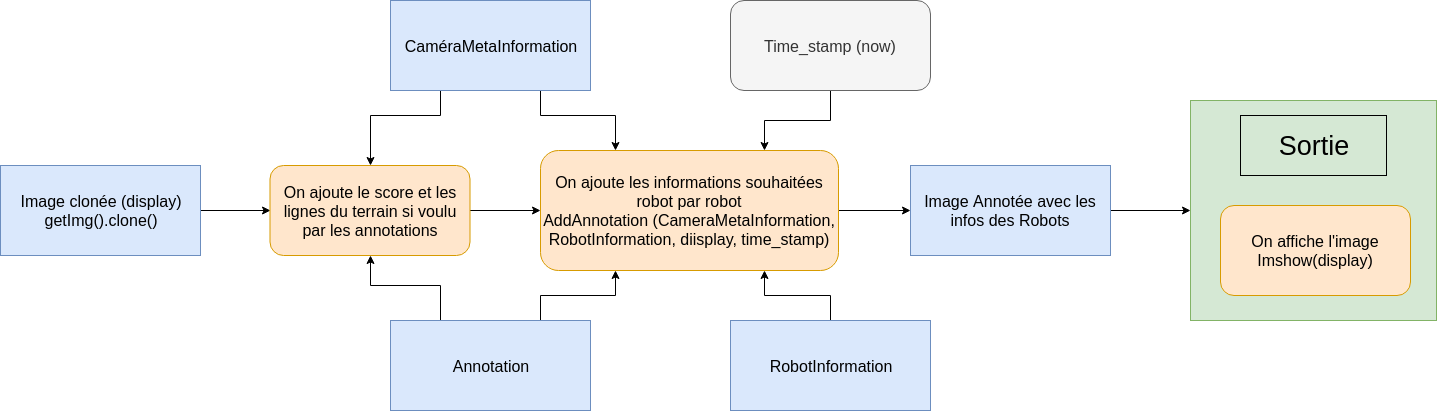
\includegraphics[scale = 0.27]{images/annotation.png}
    \caption{Annotation des images}
    \label{fig:annot}
\end{figure} 

Notre classe d'annotation comprend la fonction
\textbf{addAnnotation} globale et une fonction par annotation 
(par exemple : \textbf{annotePosition}, 
\textbf{annoteDirection} ..).
\bigskip


Dans la fonction \textbf{addAnnotation}, nous décomposons le 
message contenu par le \textbf{RobotInformation}.


Si les éléments que nous souhaitons annoter sont présents 
alors nous regardons si l'utilisateur veut afficher 
l'annotation.


Si les deux conditions sont remplies, alors nous appelons la 
fonction d'annotation adéquate. 

\section{Avantages de l'architecture}

\subsection{Ajout d'annotations}
Si dans le prolongement du projet nous voulons récupérer 
d'avantage d'informations et ajouter les annotations, notre 
architecture est adaptée.

Nous stockons déjà le message entier du robot 
(\textbf{RobotMsg}) dans la classe \textbf{RobotInformation}.
\bigskip

Ajouter des annotations comme la position des adversaires vu 
par le robot est donc assez simple. Il suffit d'ajouter une 
fonction \textbf{annoteOpponent} qui est similaire à 
l'affichage de la balle (mais avec une autre couleur et une 
autre taille).
\bigskip

Également, nous avons déjà prévu le stockage du 
\textbf{GCRobotMsg} contenant les penalty, les fautes et le 
temps restant de pénalité du robot. Il sera donc assez simple 
de les ajouter.
\bigskip

\subsection{Ajout d'équipe et de robots}
En raison de moyens limités, notre programme n'a été testé 
qu'avec deux équipes avec 2 robots contre 1. Notre 
architecture a été prévu pour tenir un nombre illimité de 
robots, ce que nous avons a testé en simulant des robots (voir
Figure~\ref{fig:scroll}).
\bigskip

 Il semble également être possible d'ajouter des équipes pour 
 la partie \textbf{annotateImage}, il se peut que toutes les 
 informations ne soient pas afficher sur l'interface.
 
Au niveau des annotations, la classe \textbf{Team} permet de 
différencier tous les robots en fonction de leur équipe et 
permet deux robots avec le même numéro mais aussi un nombre 
illimité d'équipe.

Il sera bien évidemment conseillé dans ce cas là de rajouter 
des couleurs dans le fichier 
\textit{annotation\_settings.json}.
\bigskip

Pour l'interface, l'affichage des différentes informations sur
le côté est équipé d'un scroll, qui nous permet de nous
déplacer dans l'équipe comme on peut le voir ici en simulant 
des robots.

\begin{figure}[H] 
\centering 
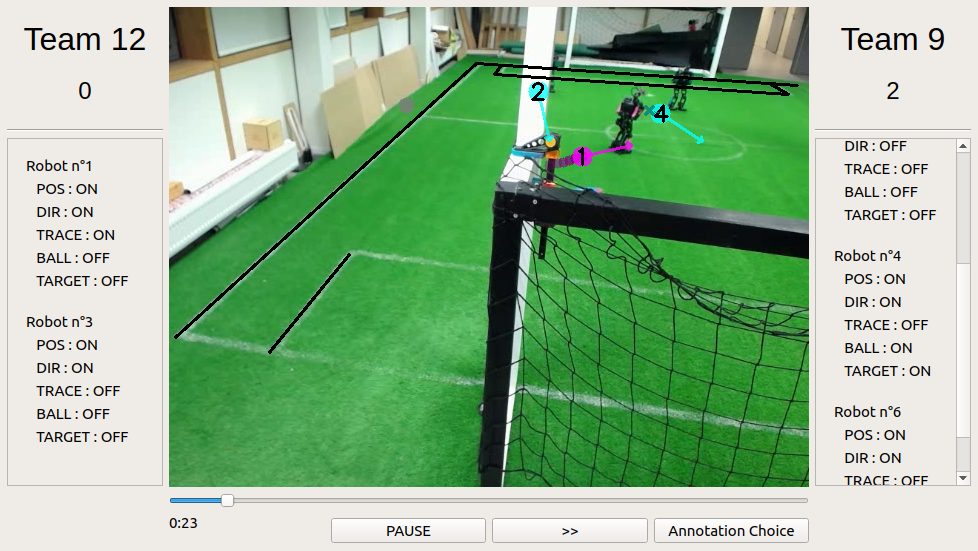
\includegraphics[scale = 0.4]{images/interfacescroll.png}
    \caption{Interface avec scroll}
    \label{fig:scroll}
\end{figure} 
\bigskip


